% !TeX spellcheck = cs_CZ
%{\tikzset{external/prefix={tikz/FYZII/}}
% \tikzset{external/figure name/.add={ch36_}{}}
%---------------------------------------------------------------------------------------------------
% file fey2ch36.tex
%---------------------------------------------------------------------------------------------------
%=========================== Kapitola Feromagnetizmus ==============================================
\chapter{Feromagnetizmus}\label{fyz:IIchapXXXVI}
\minitoc
  \section{Magnetizační proudy}\label{fyz:IIchapXXXVIsecI}
  \section{Pole H}\label{fyz:IIchapXXXVIsecII}
  \section{Magnetizační křivka}\label{fyz:IIchapXXXVIsecIII}
  \section{Indukčnost ocelových jader}\label{fyz:IIchapXXXVIsecIV}
  \section{Elektromagnety}\label{fyz:IIchapXXXVIsecV}
  \section{Spontánní magnetizace}\label{fyz:IIchapXXXVIsecVI}
  \section{Příklady a cvičení}\label{fyz:IIchapXXXVIsecVII}

    \begin{figure}[ht!] %\ref{fyz_fig831}
      \centering
      \begin{tabular}{c}
        \subfloat[ ]{\label{fyz_fig831a}
          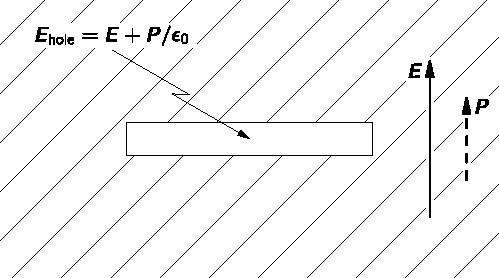
\includegraphics[width=0.7\linewidth]{fyz_fig831a.pdf}}               \\
        \subfloat[ ]{\label{fyz_fig831b}
          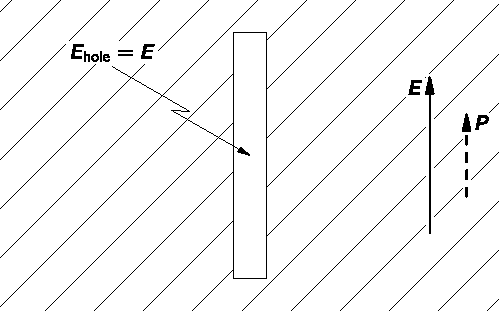
\includegraphics[width=0.7\linewidth]{fyz_fig831b.pdf}}               \\
        \subfloat[ ]{\label{fyz_fig831c}
          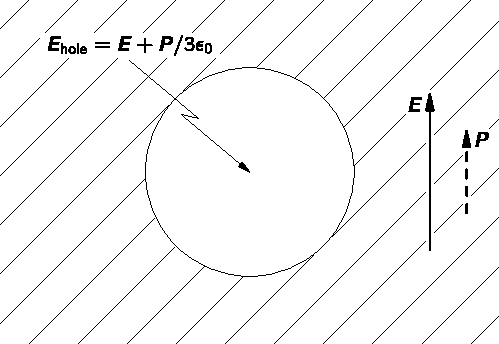
\includegraphics[width=0.7\linewidth]{fyz_fig831c.pdf}}
      \end{tabular}
      \caption{
               (\cite[s.~748]{Feynman02})}
      \label{fyz_fig831}
    \end{figure}

    \begin{figure}[ht!] %\ref{fyz_fig832}
      \centering
      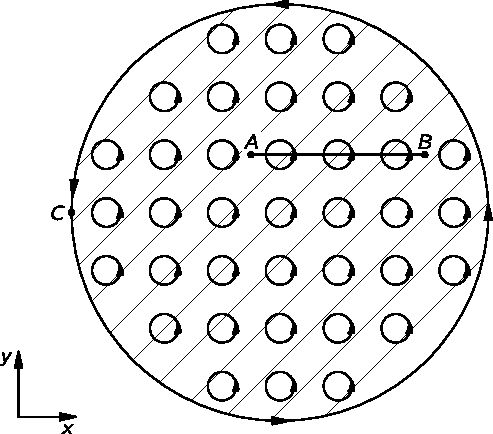
\includegraphics[width=0.7\linewidth]{fyz_fig832.pdf}
      \caption{
               (\cite[s.~707]{Feynman02})}
      \label{fyz_fig832}
    \end{figure}
    
    \begin{figure}[ht!] %\ref{fyz_fig833}
      \centering
      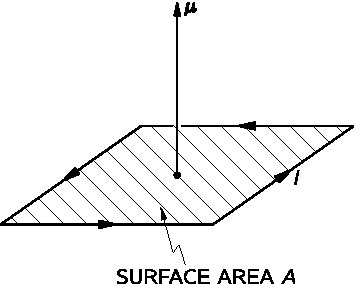
\includegraphics[width=0.7\linewidth]{fyz_fig833.pdf}
      \caption{
               (\cite[s.~707]{Feynman02})}
      \label{fyz_fig833}
    \end{figure}
    
    \begin{figure}[ht!] %\ref{fyz_fig834}
      \centering
      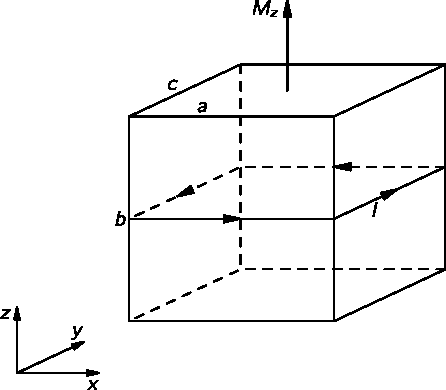
\includegraphics[width=0.7\linewidth]{fyz_fig834.pdf}
      \caption{
               (\cite[s.~707]{Feynman02})}
      \label{fyz_fig834}
    \end{figure}
    
    \begin{figure}[ht!] %\ref{fyz_fig835}
      \centering
      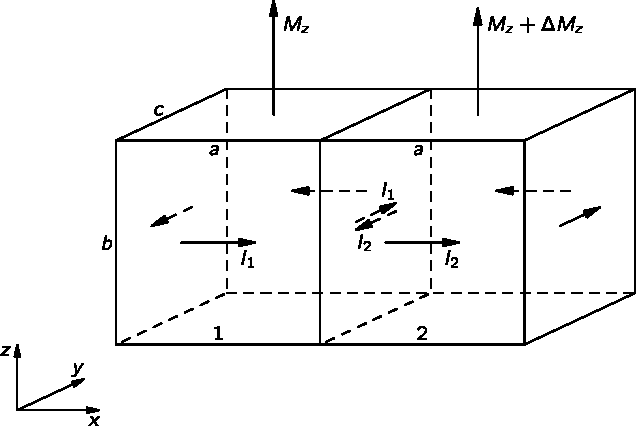
\includegraphics[width=0.7\linewidth]{fyz_fig835.pdf}
      \caption{
               (\cite[s.~707]{Feynman02})}
      \label{fyz_fig835}
    \end{figure}
    
    \begin{figure}[ht!] %\ref{fyz_fig836}
      \centering
      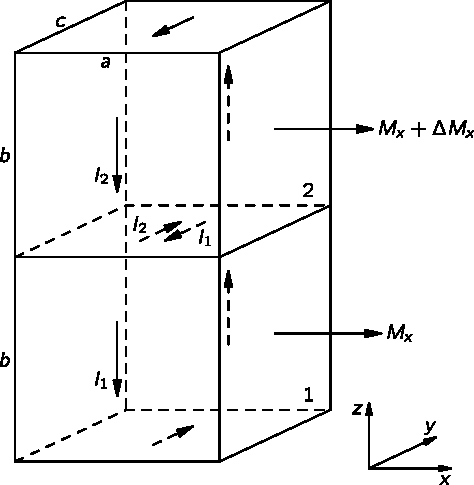
\includegraphics[width=0.7\linewidth]{fyz_fig836.pdf}
      \caption{
               (\cite[s.~707]{Feynman02})}
      \label{fyz_fig836}
    \end{figure}

    \begin{figure}[ht!] %\ref{fyz_fig837}
      \centering
      \begin{tabular}{c}
        \subfloat[ ]{\label{fyz_fig837a}
          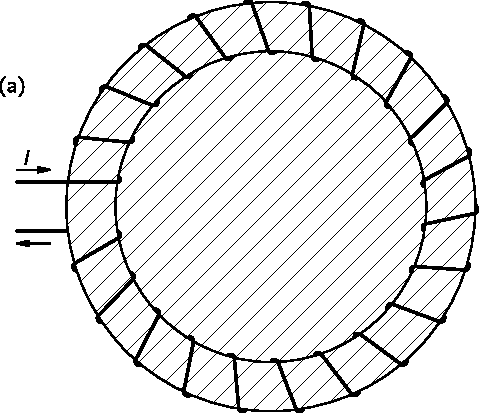
\includegraphics[width=0.7\linewidth]{fyz_fig837a.pdf}}               \\
        \subfloat[ ]{\label{fyz_fig837b}
          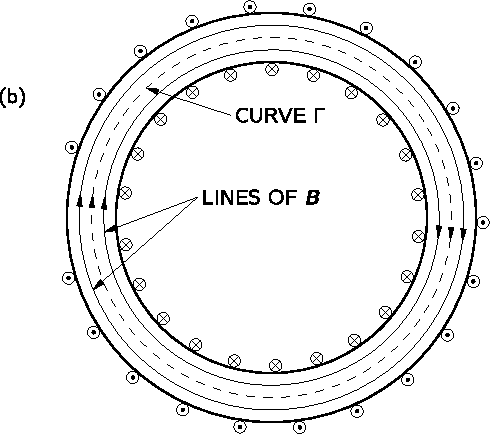
\includegraphics[width=0.7\linewidth]{fyz_fig837b.pdf}}
      \end{tabular}
      \caption{
               (\cite[s.~748]{Feynman02})}
      \label{fyz_fig837}
    \end{figure}

    \begin{figure}[ht!] %\ref{fyz_fig838}
      \centering
      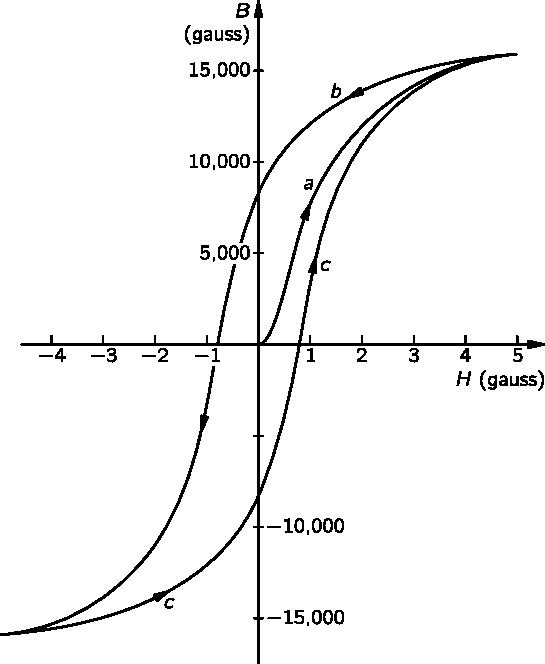
\includegraphics[width=0.7\linewidth]{fyz_fig838.pdf}
      \caption{
               (\cite[s.~707]{Feynman02})}
      \label{fyz_fig838}
    \end{figure}

    \begin{figure}[ht!] %\ref{fyz_fig839}
      \centering
      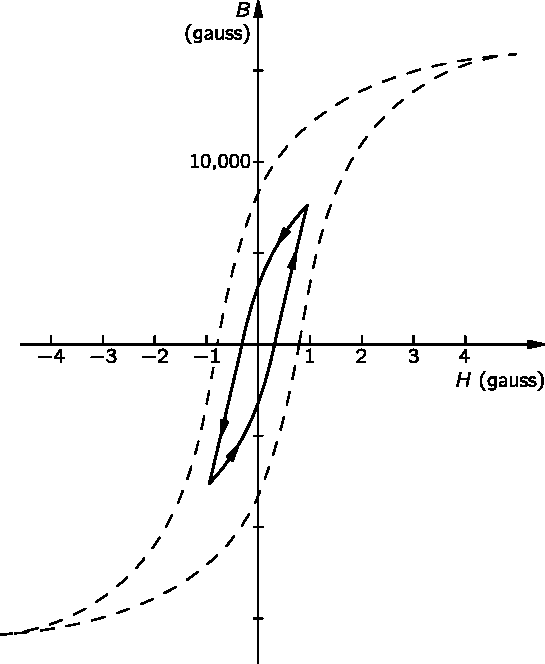
\includegraphics[width=0.7\linewidth]{fyz_fig839.pdf}
      \caption{
               (\cite[s.~707]{Feynman02})}
      \label{fyz_fig839}
    \end{figure}

    \begin{figure}[ht!] %\ref{fyz_fig840}
      \centering
      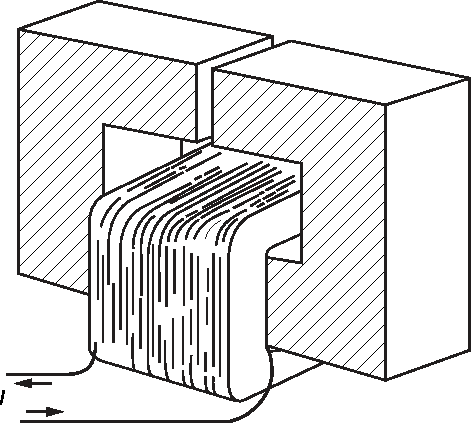
\includegraphics[width=0.7\linewidth]{fyz_fig840.pdf}
      \caption{
               (\cite[s.~707]{Feynman02})}
      \label{fyz_fig840}
    \end{figure}
    
    \begin{figure}[ht!] %\ref{fyz_fig841}
      \centering
      \begin{tabular}{c}
        \subfloat[ ]{\label{fyz_fig841a}
          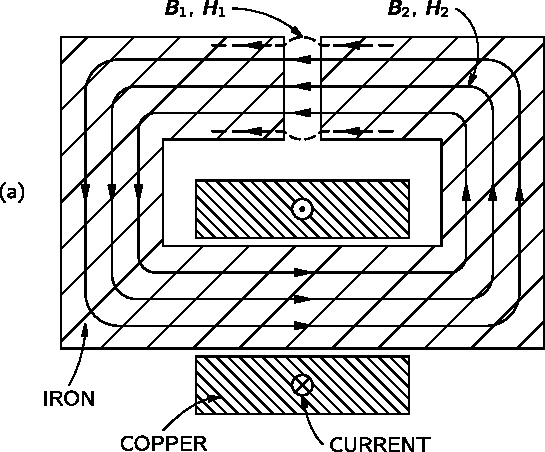
\includegraphics[width=0.7\linewidth]{fyz_fig841a.pdf}}               \\
        \subfloat[ ]{\label{fyz_fig841b}
          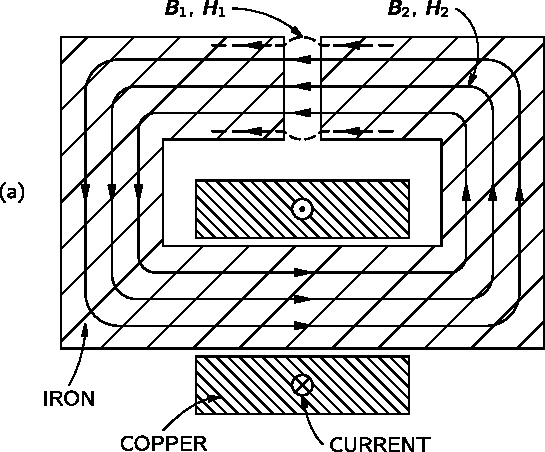
\includegraphics[width=0.7\linewidth]{fyz_fig841b.pdf}}
      \end{tabular}
      \caption{
               (\cite[s.~748]{Feynman02})}
      \label{fyz_fig841}
    \end{figure}

    \begin{figure}[ht!] %\ref{fyz_fig842}
      \centering
      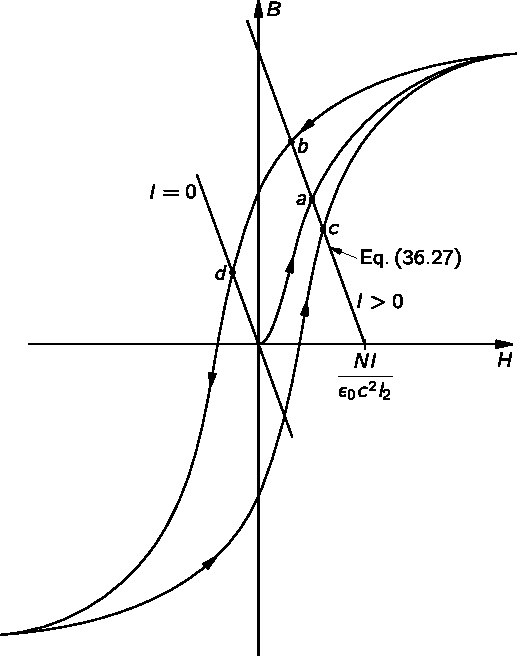
\includegraphics[width=0.7\linewidth]{fyz_fig842.pdf}
      \caption{
               (\cite[s.~707]{Feynman02})}
      \label{fyz_fig842}
    \end{figure}

    \begin{figure}[ht!] %\ref{fyz_fig843}
      \centering
      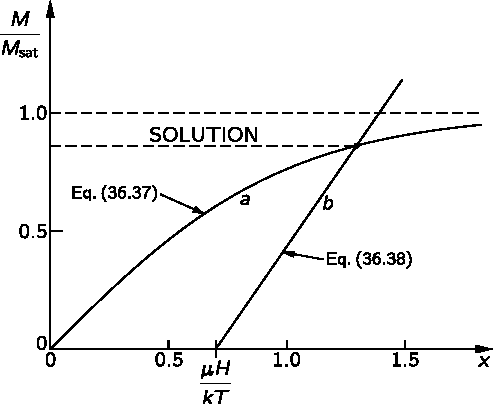
\includegraphics[width=0.7\linewidth]{fyz_fig843.pdf}
      \caption{
               (\cite[s.~707]{Feynman02})}
      \label{fyz_fig843}
    \end{figure}

    \begin{figure}[ht!] %\ref{fyz_fig844}
      \centering
      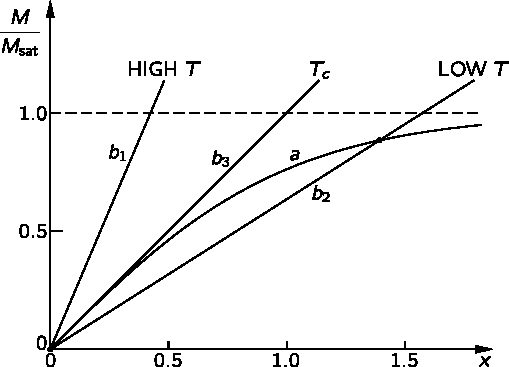
\includegraphics[width=0.7\linewidth]{fyz_fig844.pdf}
      \caption{
               (\cite[s.~707]{Feynman02})}
      \label{fyz_fig844}
    \end{figure}

    \begin{figure}[ht!] %\ref{fyz_fig845}
      \centering
      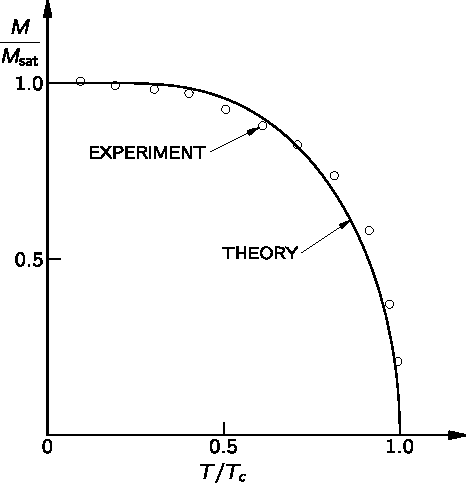
\includegraphics[width=0.7\linewidth]{fyz_fig845.pdf}
      \caption{
               (\cite[s.~707]{Feynman02})}
      \label{fyz_fig845}
    \end{figure}
    
%} %tikzset
%---------------------------------------------------------------------------------------------------
\printbibliography[title={Seznam literatury},heading=subbibliography]
\addcontentsline{toc}{section}{Seznam literatury}